\chapter{Дополнительные иллюстрации}\label{app:1}

\begin{figure}[ht]
	\,
	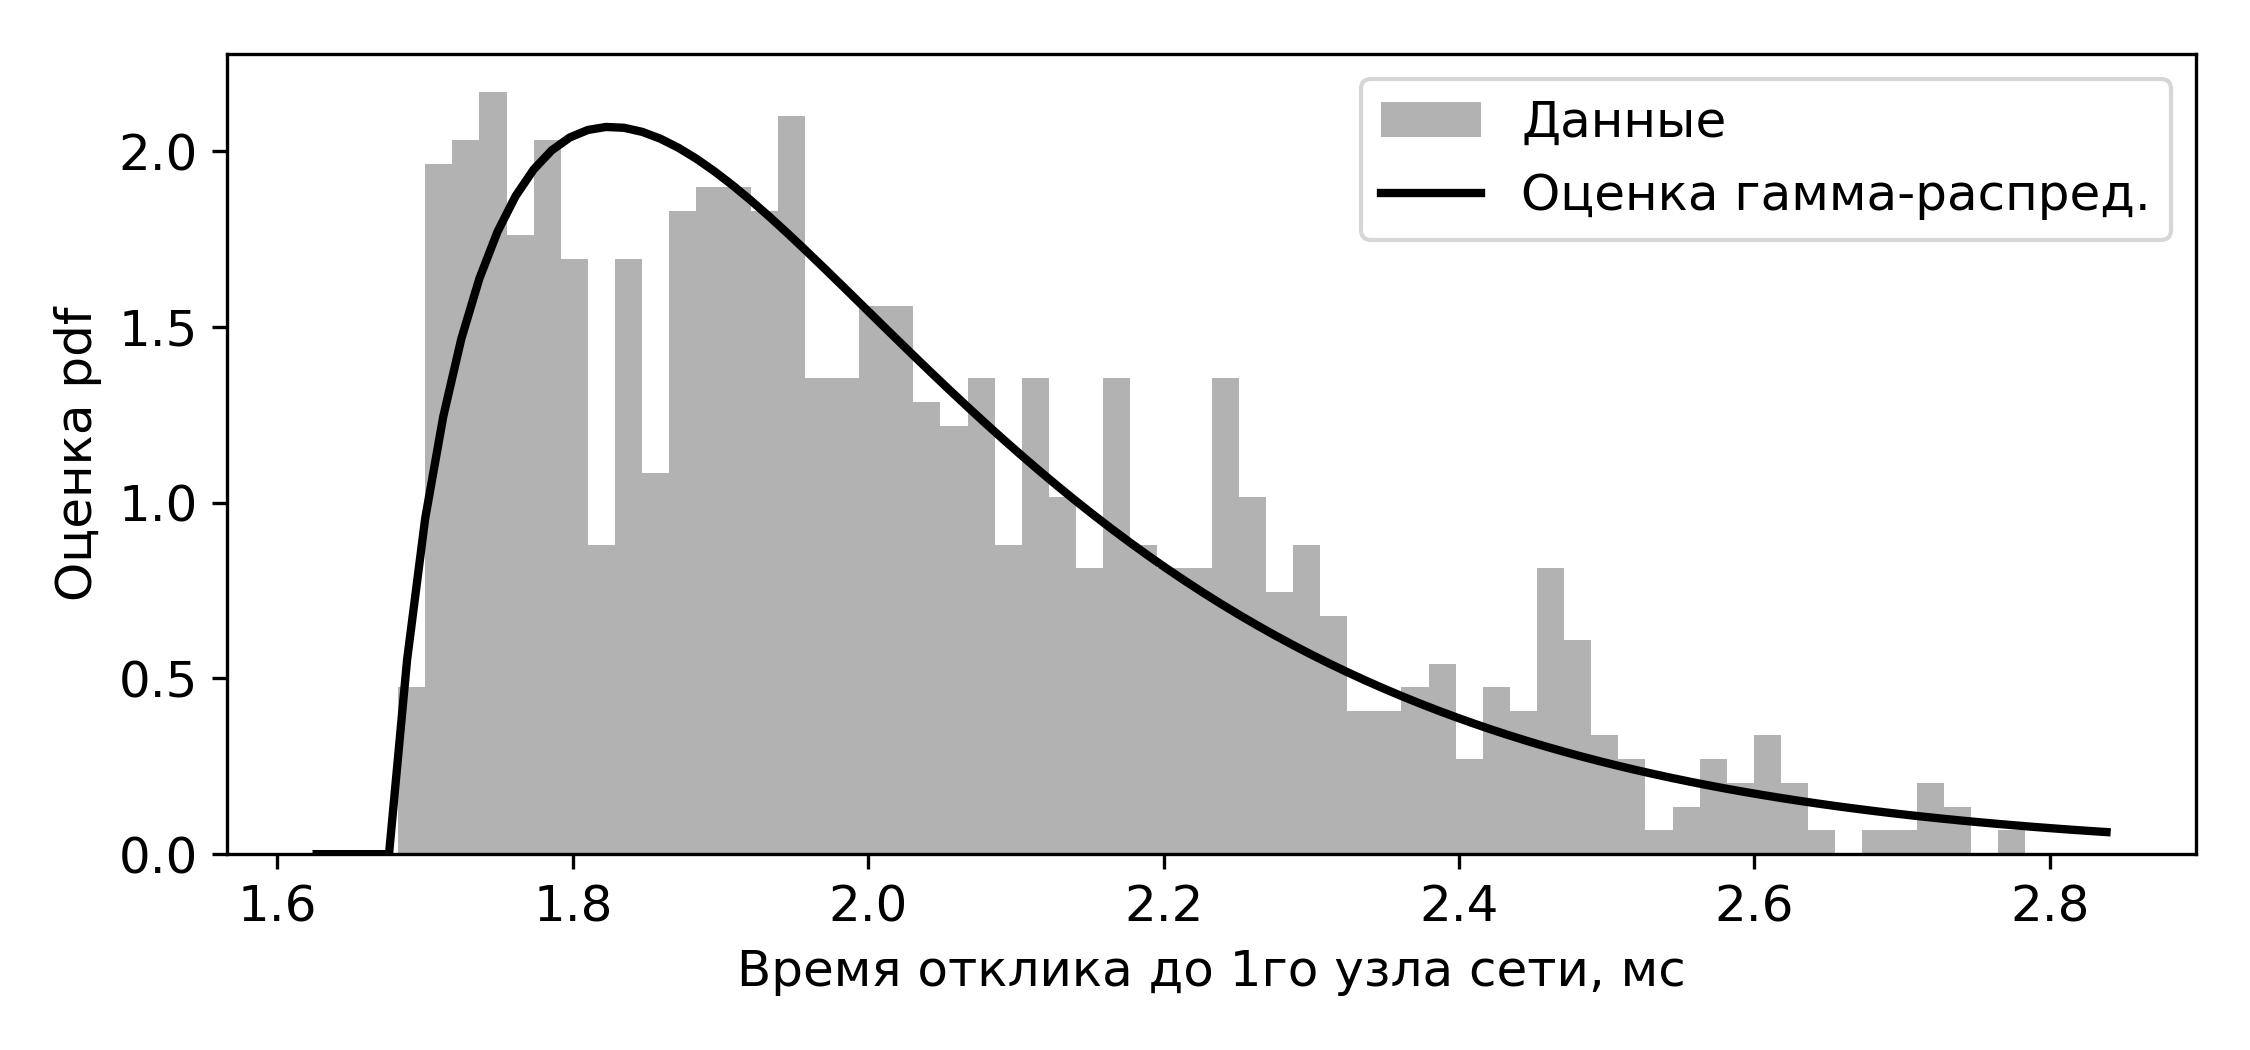
\includegraphics[width=0.8\textwidth]{images/calib/example_kde}
	\caption{Пример получаемого приближения pdf для устройства типа <<system: V1>> с использованием гамма-распределения}
	\label{fig:examplekde}
\end{figure}


\chapter{Листинги программного кода}\label{app:A}

\begin{ListingEnv}[!h]% настройки floating аналогичны окружению figure
    \captiondelim{ } % разделитель идентификатора с номером от наименования
    \caption{Основной фрагмент программы calibration.py, используемый для калибровки данных из системы RIPE Atlas}\label{lst:calib}
    % окружение учитывает пробелы и табуляции и применяет их в сответсвии с настройками
    \begin{lstlisting}[language={Python}]
	import pandas as pd
	import numpy as np
	from scipy.stats import lognorm, skewnorm
	
	def make_calibration(data_ref, data_uncalib, pdf_type='gamma'):
	'''
	Калибрует данные в data_uncalib базируясь на данных data_ref. 
	Обычно data_ref - это даннные с устройств system V3
	'''
		if pdf_type=='gamma':
			dstr = gamma
		elif pdf_type=='lognorm':
			dstr = lognorm
		else:
			print('Unsupported pdf_type')
		return None
		ref_params = dstr.fit(data_ref)
		uncalib_params = dstr.fit(data_uncalib)
		
		cdf_values = dstr.cdf(data_uncalib, *uncalib_params)
		data_calibr = dstr.ppf(cdf_values, *ref_params)
		
		return data_calibr
	
    \end{lstlisting}
\end{ListingEnv}%


\chapter{Дополнительные табличные данные}\label{app:B}

%Пример длинной таблицы с записью продолжения по ГОСТ 2.105:

\begingroup
\centering
\small
\captionsetup[table]{skip=7pt} % смещение положения подписи
\begin{longtable}[c]{|>{\centering\arraybackslash}p{1.2cm}|>{\centering\arraybackslash}p{1.2cm}|>{\centering\arraybackslash}p{1.8cm}|>{\centering\arraybackslash}p{1.2cm}|>{\centering\arraybackslash}p{1.2cm}|>{\centering\arraybackslash}p{3.8cm}|>{\centering\arraybackslash}p{3.3cm}|}
	\caption{Аномальные узлы, обнаруженные в ходе анализа данных о времени отклика. $RTT_{m}$ - оценка времени отклика моделью, $RTT_{obs}$ - результат измерений}\label{tab:anomalies}% label всегда желательно идти после caption
	\\[-0.45\onelineskip]
	\hline
	RIPE id & ASN & Удаление, км & $RTT_{m}$, мс & $RTT_{obs}$, мс & Название AS  & Город \\ \hline
	\endfirsthead%
	\caption*{Продолжение таблицы~\thetable}                                    \\[-0.45\onelineskip]
	\hline
	RIPE id & ASN & Удаление, км & $RTT_{m}$, мс & $RTT_{obs}$, мс & Название AS  & Город \\ \hline
	\endhead
	\hline
	\endfoot
	\hline
	\endlastfoot
	10249 & 8359 & 1717,5 & 32,8 & 58,7 & MTS & Тюмень  \\
	11072 & 56330 & 1736,5 & 33,1 & 48,5 & KURGAN-AS  & Курган  \\
	13533 & 61400 & 4,8 & 7,0 & 20,6 & NETRACK-AS &  Москва  \\ 
	14608 & 20485 & 467,9 & 13,9 & 25,7 & TRANS- TELECOM & Воронеж  \\
	16854 & 201285 & 90,5 & 8,3 & 31,8 & KIRZHACH- TELECOM & Киржач  \\ 
	18641 & 33871 & 2890,4 & 50,5 & 62,7 & Norilsk-Telecom-AS & Норильск  \\ 
	19921 & 41668 & 723,0 & 17,8 & 36,2 & ERTH-KAZAN-AS & Казань  \\ 
	20727 & 41668 & 724,4 & 17,8 & 36,2 & ERTH-KAZAN-AS & Казань  \\ 
	22712 & 31213 & 612,3 & 16,1 & 77,8 & MF-NWGSM-AS & Псков  \\
	26966 & 6856 & 573,1 & 15,5 & 24,7 & IC-VORONEZH-AS &  Белгород  \\
	27300 & 50071 & 989,6 & 21,8 & 39,2 & SRDV-AS &  Северодвинск  \\ 
	28137 & 39028 & 781,0 & 18,7 & 38,2 & ULSK-AS &  Димитровград  \\ 
	28543 & 210616 & 1219,6 & 25,3 & 37,3 & SIBMEDVED-AS & Новороссийск  \\
	28622 & 51004 & 6639,5 & 107,1 & 117,3 & SCTS-AS &  Южно-Сахалинск  \\ 
	28664 & 12683 & 1342,4 & 27,2 & 39,9 & STATEL-AS &  Минеральные воды  \\
	31468 & 206012 & 373,4 & 12,5 & 23,1 & AXIOSTV-AS & Липецк  \\
	33318 & 8359 & 19,9 & 7,2 & 40,3 & MTS & Москва  \\
	%\end{tabular}
\end{longtable}

\normalsize% возвращаем шрифт к нормальному
\endgroup


\begin{comment}

\section{Очередной подраздел приложения}\label{app:B5}

Нужно больше подразделов приложения!

\section{И ещё один подраздел приложения}\label{app:B6}

Нужно больше подразделов приложения!

\clearpage
\refstepcounter{chapter}
\addcontentsline{toc}{appendix}{\protect\chapternumberline{\thechapter}Чертёж детали}

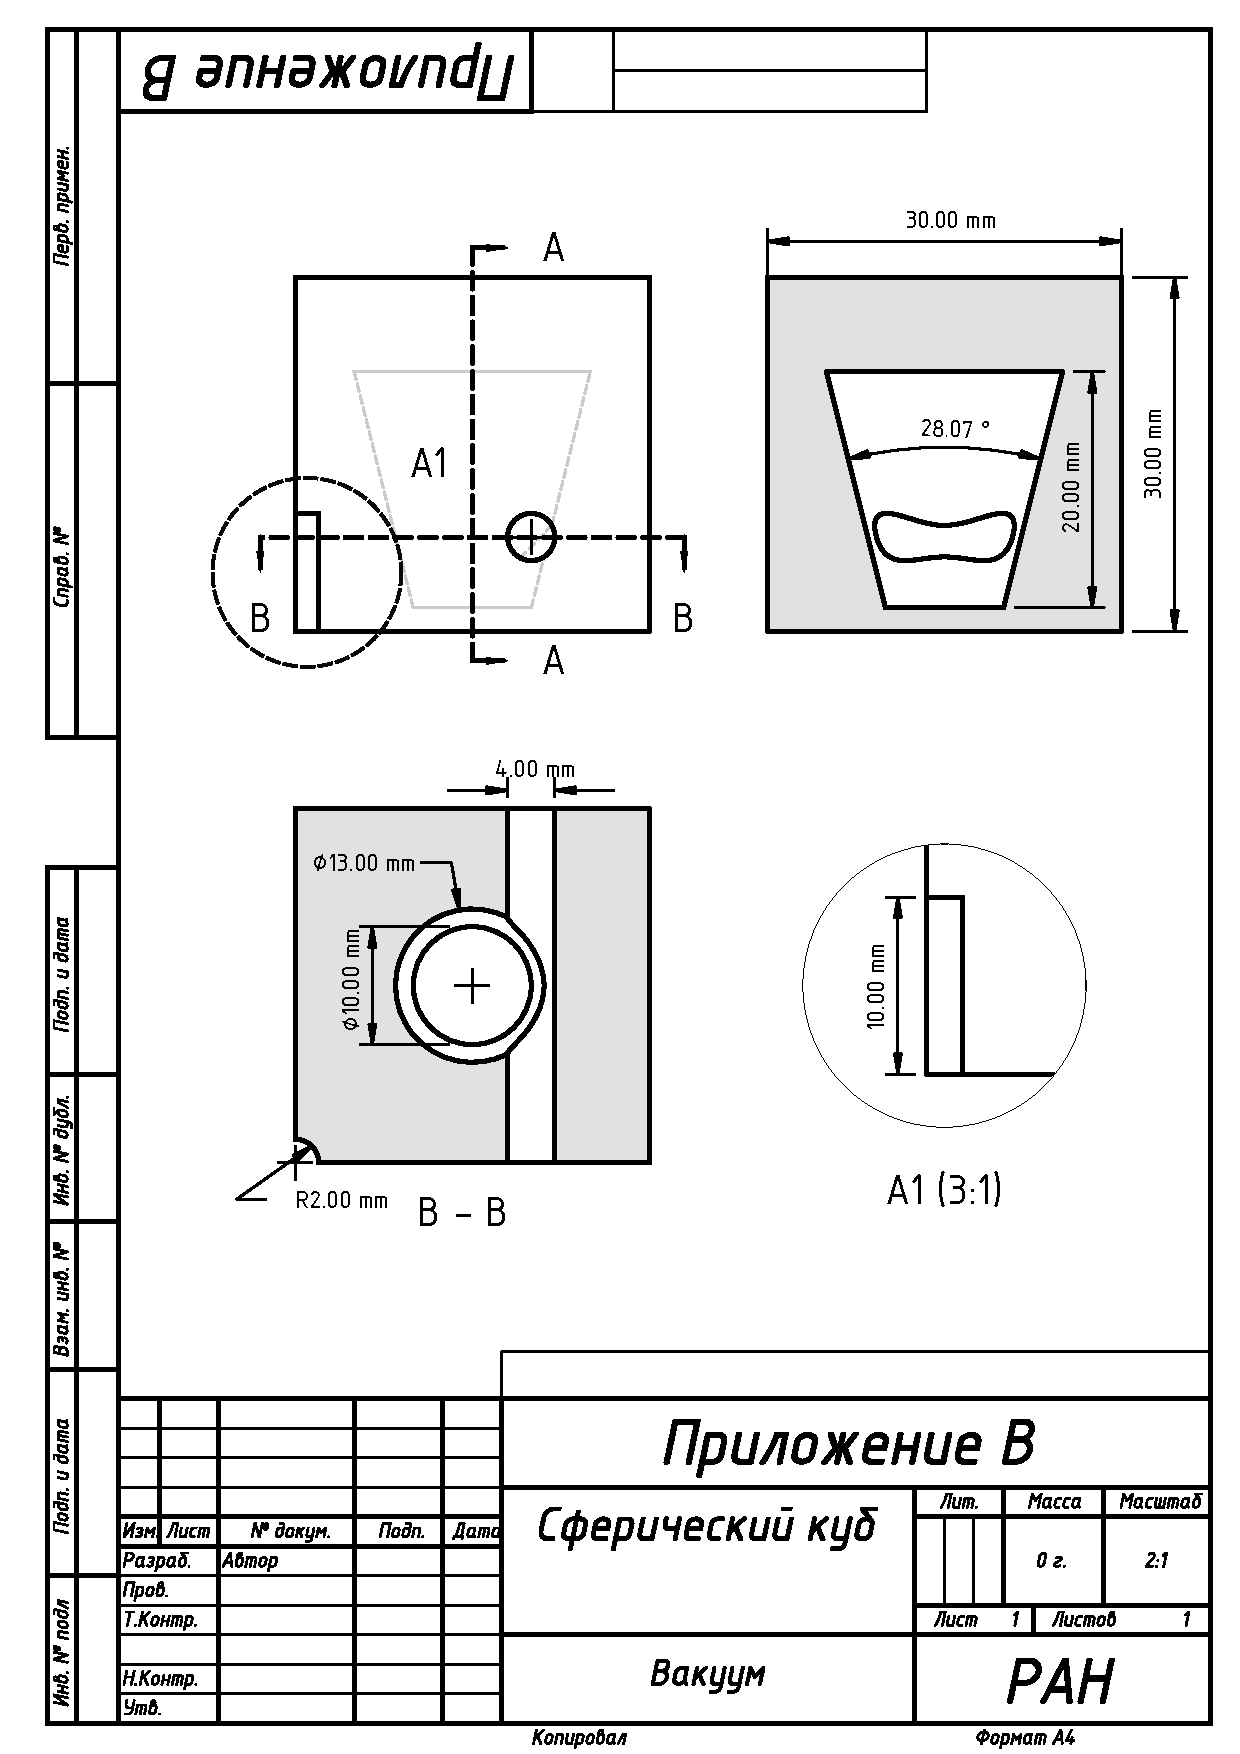
\includepdf[pages=-]{Dissertation/images/drawing.pdf}

\end{comment}